\chapter{Boundary Conditions}

\section{Radiation}
The net radiation heat flux from surface 1 to surface 2 using grey body radiation can be calculated as 
\begin{equation}
	\dot{Q}_{1 \rightarrow 2} = A_1 F_{1 \rightarrow 2} E_1 -  A_2 F_{2 \rightarrow 1} E_2.
\end{equation}
using the formula for emission of grey bodies
\begin{equation}
	E_i = \epsilon_i \sigma T_i^4 
\end{equation}
and the reciprocity rule for configuration factors $A_1 F_{1 \rightarrow 2} = A_2 F_{2 \rightarrow 1}$ we can write
\begin{equation}
	\dot{Q}_{1 \rightarrow 2} = \sigma A_1 F_{1 \rightarrow 2} \left(\epsilon_1 T1^4 - \epsilon_2 T_2^4\right)
\end{equation}
and $\dot{Q}_{1 \rightarrow 2} = -\dot{Q}_{2 \rightarrow 1}$.
Given two line segments as seen in Fig.~\ref{fig:radiation}
%---------------------------------------------------------------------------------------------------------------
\begin{figure}[H]
	\centering
	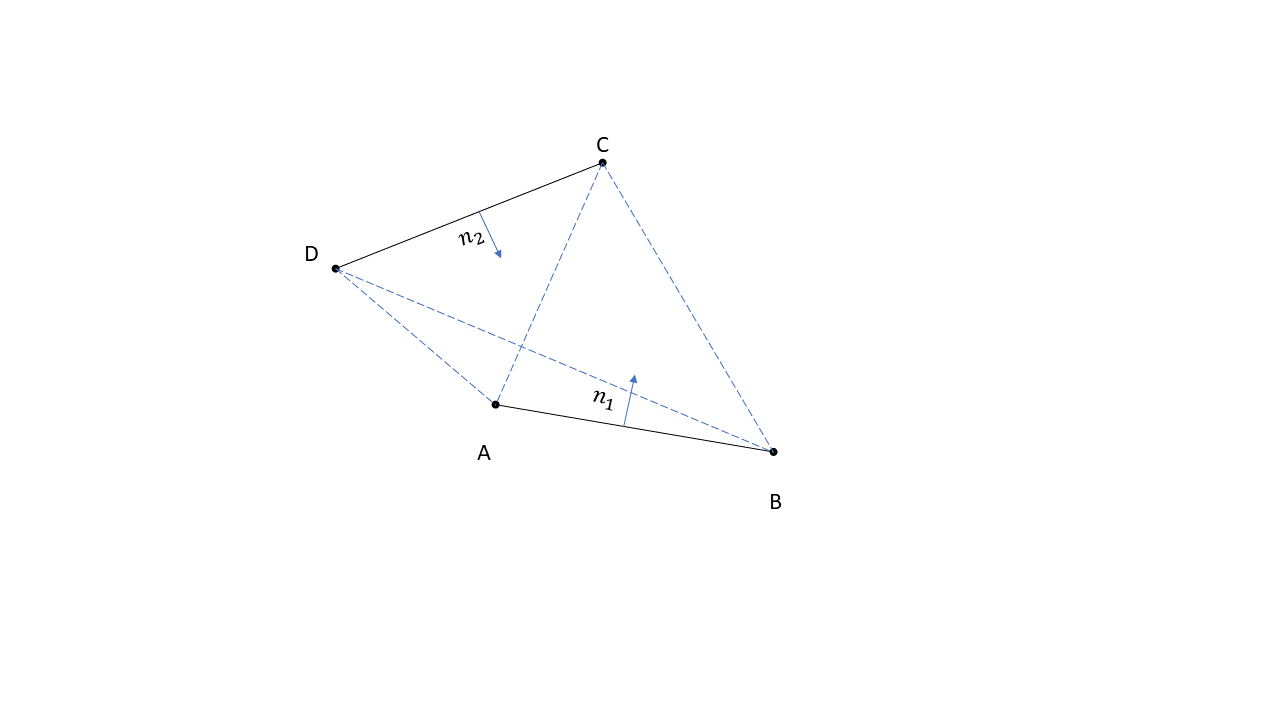
\includegraphics[trim= 8cm 5cm 13cm 3.5cm ,clip,width=0.6\textwidth]{figures/radiation.png}
	\caption{Radiation.}
	\label{fig:radiation}
\end{figure}
%---------------------------------------------------------------------------------------------------------------
the configuration factor from surface $\overline{\mm{AB}}$ to surface $\overline{\mm{CD}}$ can be calculated as
\begin{equation}
	F_{\overline{\mm{AB}} \rightarrow \overline{\mm{CD}}} = \frac{\overline{\mm{AC}} + \overline{\mm{BD}} - \overline{\mm{AD}} - \overline{\mm{BC}}}{2 \overline{\mm{AB}}}
\end{equation}
where $\overline{\mm{XY}}$ is the distance from $\mm{X}$ to $\mm{Y}$.
The total heat flux from or to a single surface is the sum of the heat fluxes to other surfaces plus the heat flux to the background
\begin{equation}
	\dot{Q}_{tot} = \sigma A_1 \left\{\epsilon_1 T_1^4 \sum_i F_{1 \rightarrow i} - \sum_i \epsilon_i F_{1 \rightarrow i}  T_i^4 \right\} + \dot{Q}_{backgr}
\end{equation}

In terms of boundary conditions we ca write
\begin{equation}
	\lambda \left(\vec{n} \cdot \nabla T \right) = \frac{\dot{Q}_{1 \rightarrow 2}}{A_1} = \sigma F_{1 \rightarrow 2} \left(\epsilon_1 T1^4 - \epsilon_2 T_2^4\right)
\end{equation}
and using a Taylor series
\begin{equation}
	\mm{T}\left[ T^4 \right] \approx T_0^4 + 4 T_0^3 \left(T - T_0 \right) =  4 T_0^3 T - 3 T_0^4
\end{equation}
and the shorthand $\tilde{\epsilon}_i = \epsilon_i \sigma F_{1 \rightarrow 2}$ we get
\begin{equation}
	\lambda \left(\vec{n} \cdot \nabla T \right)  - 4 \tilde{\epsilon}_1 T_{1, 0}^3 T_1 + 4 \tilde{\epsilon}_2 T_{2, 0}^3 T_2   = 3 \tilde{\epsilon}_2 T_{2, 0}^4 - 3 \tilde{\epsilon}_1 T_{1, 0}^4.
\end{equation}